\renewcommand{\thislecture}{8 }

%
% Cover page
%

\title[Neutrino Physics / Lecture \thislecture]
{
  {\huge \color{yellow} Neutrino Physics - Lecture \thislecture} \\
  {\it Resonance Neutrino-Production}\\
}

\author[C.Andreopoulos] {
  Professor Costas Andreopoulos\inst{1,2}
}
\institute[Liverpool/STFC-RAL] {
   \inst{1} University of Liverpool,
   \inst{2} STFC Rutherford Appleton Laboratory\\
   \vspace{0.5cm}
   {\it {\color{magenta} A post-graduate student lecture course}}\\
   \vspace{0.2cm}
}
\date{\today}

\titlegraphic{
  
\includegraphics[height=25px]{./images/logo/liverpool.png}
  \hspace{3px}
  
\includegraphics[height=30px]{./images/logo/ral.png}
}

	



\begin{frame}[plain]
  \titlepage
\end{frame}

%
% Outline
%

\begin{frame}{Outline for Lecture \thislecture}


\end{frame}

%
%
%
\begin{frame}{Single-$\pi$ production}

  {\scriptsize
    Dominant process in the region of
    transition from the non-perturbative to perturbative regime.\\
    Important process for oscillation physics (both as a signal and background).
    \begin{itemize}
     \item In DUNE, resonance events cntribute $\sim$30\% to the CC inclusive rate.\\
     \item In T2K/HyperK, single-pion events can mimic single-ring (QE-enhanced) signal events\\
     \item NC1$\pi^{0}$ an important background for $\nu_{e}$/$\bar{\nu}_{e}$ appearance\\
   \end{itemize}
  }
  \begin{columns}
    \begin{column}{0.38\textwidth}
      \begin{center}
        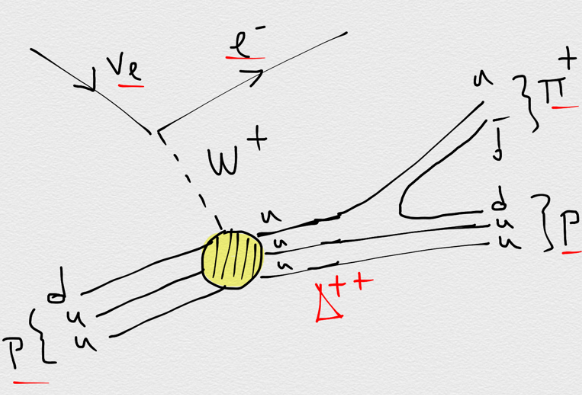
\includegraphics[width=0.80\textwidth]{./images/nuint/feyn/ccDelta1pi_feynman_diagram_0}\\
        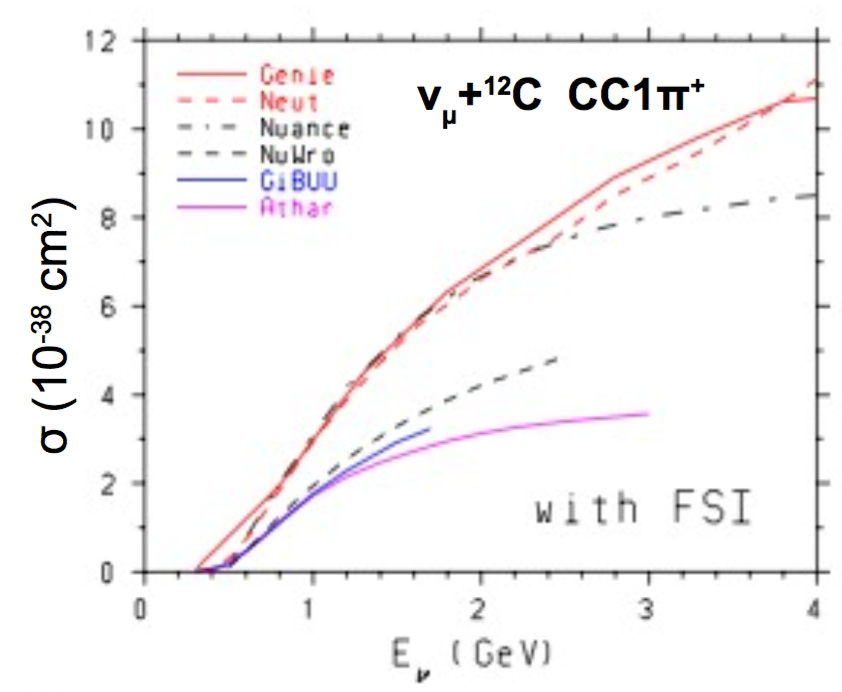
\includegraphics[width=0.90\textwidth]{./images/nuint/ccpi/sig1pi_various_models}\\
      \end{center}
    \end{column}
    \begin{column}{0.62\textwidth}
     \begin{center}
        {\scriptsize \color{cadmiumred}
          Number of T2K $\mu$-like single-ring events to date\\
          in the neutrino beam mode (FHC):\\
        }
        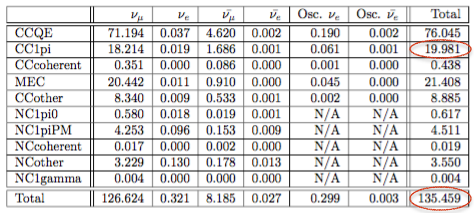
\includegraphics[width=0.80\textwidth]{./images/nuint/other/T2KFHC1RmuRun1to7_annotated}\\
        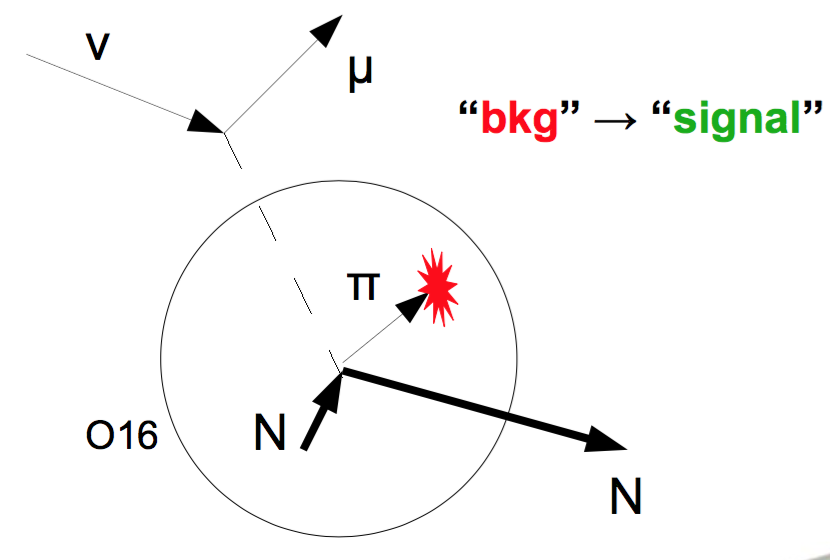
\includegraphics[width=0.45\textwidth]{./images/nuint/feyn/single_pi_bkg_to_signal}\\
     \end{center}
    \end{column}
  \end{columns}

\end{frame}

%
%
%
\begin{frame}{Single-$\pi$ production}

{\scriptsize
  First recent (flux integrated double-differential) CC1$\pi^{\pm}$
  (predominantly CC1$\pi^{+}$) measurement was performed by MiniBooNE
  [Phys.Rev.D83, 052007 (2011)]
}

  \begin{columns}
    \begin{column}{0.62\textwidth}
      \begin{center}
         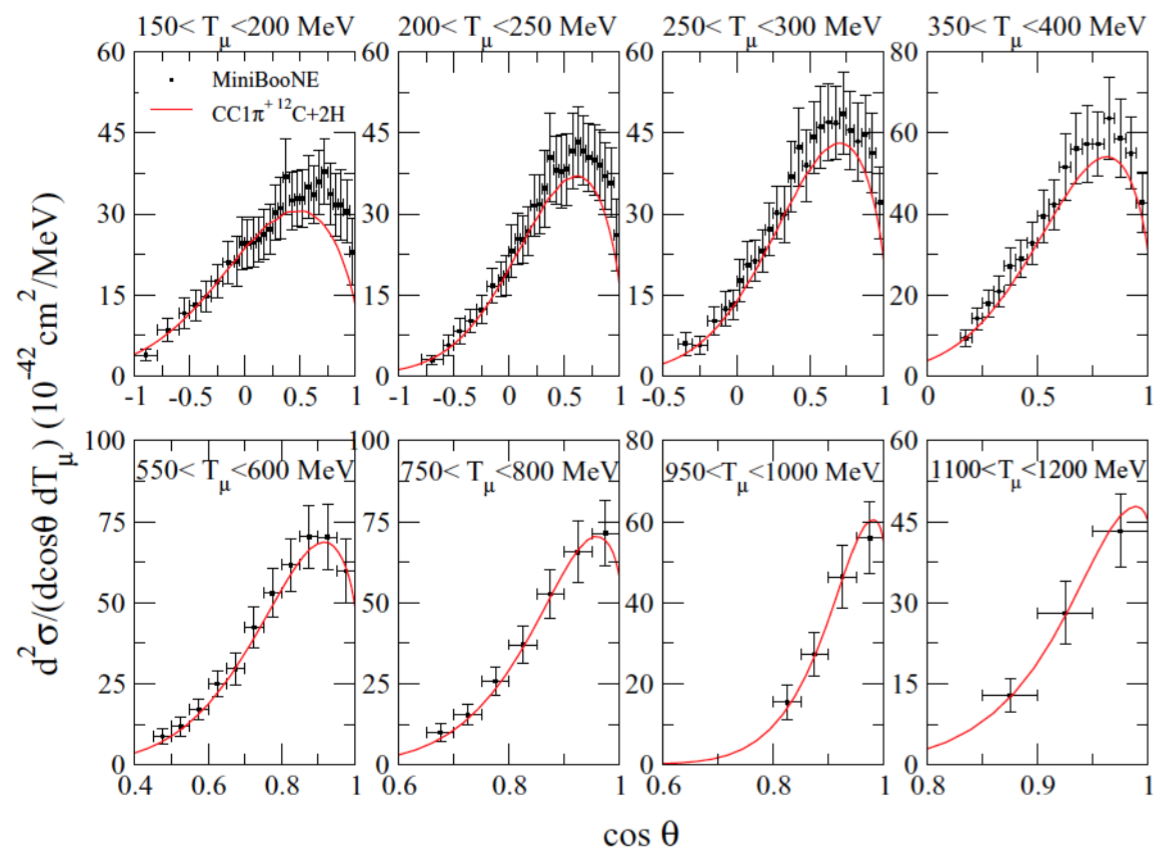
\includegraphics[width=0.98\textwidth]{./images/nuint/ccpi/mb_cc1pip.png}\\
         {\scriptsize [Phys.Rev.C90,025501(2014)]}
      \end{center}
    \end{column}
    \begin{column}{0.38\textwidth}
     {\scriptsize
      Differential cross-section in muon kinematics
      (muon kinetic energy $T_{\mu}$ and muon scattering angle $\theta_{\mu}$).\\
      \vspace{0.3cm}
      Reasonable agreement is obtained with several models.\\
     }
    \end{column}
  \end{columns}

\end{frame}

%
%
%
\begin{frame}{The single-$\pi$ puzzle}

{\scriptsize
 But MiniBooNE data in terms of pion kinematics very hard to understand within any model.\\
 \vspace{0.3cm}
 Shape of MiniBooNE $T_{\pi}$ distribution seems to prefer the absence of FSI effects!\\
}

  \begin{columns}
    \begin{column}{0.60\textwidth}
      \begin{center}
        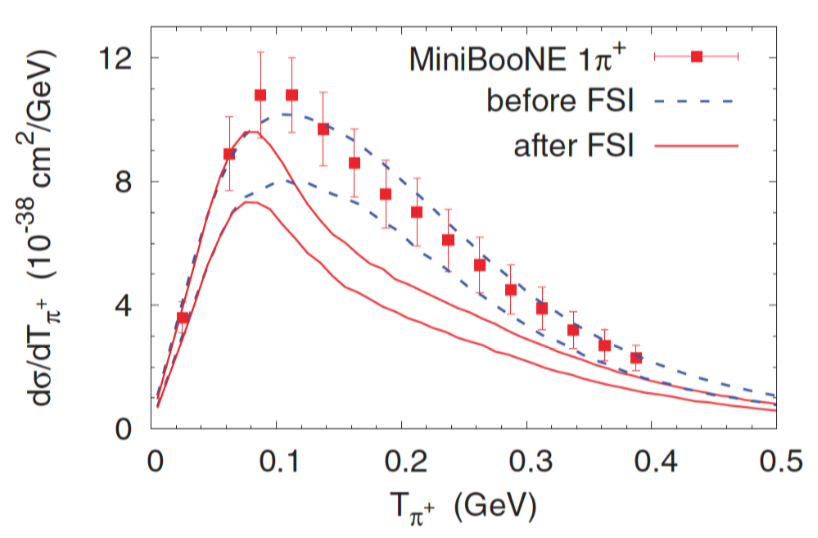
\includegraphics[width=0.99\textwidth]{./images/nuint/ccpi/mb_cc1pip_w_wo_fsi.png}\\
        {\scriptsize [Phys.Rev.C87, 014602 (2013)]}
      \end{center}
    \end{column}
    \begin{column}{0.40\textwidth}
      \begin{center}
         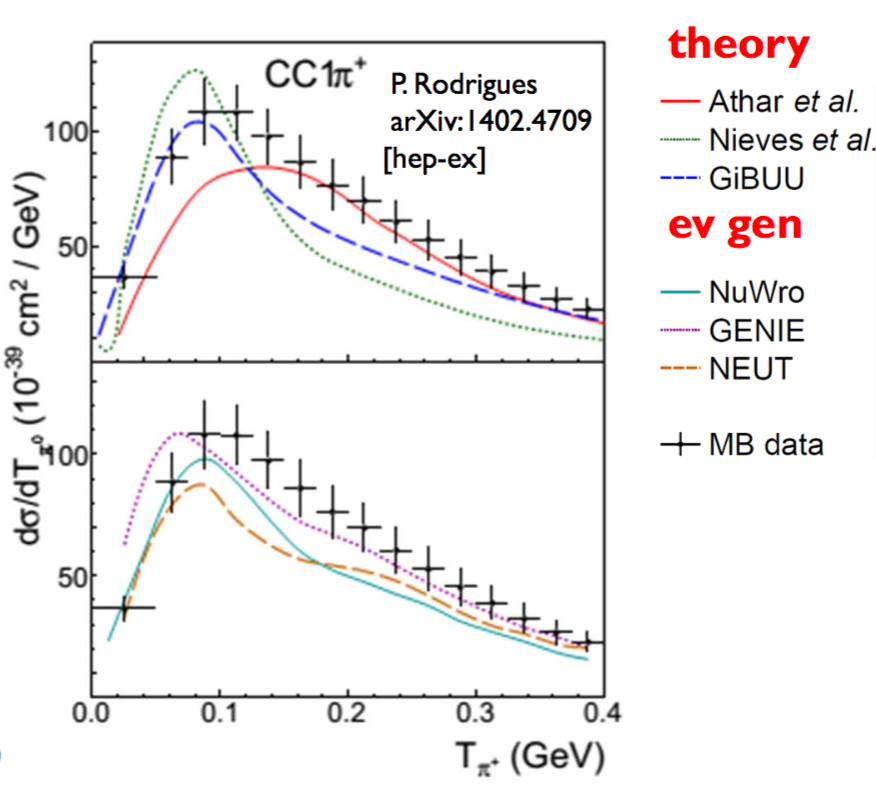
\includegraphics[width=0.98\textwidth]{./images/nuint/ccpi/mb_cc1pi_many_models.png}\\
         {\scriptsize [arXiv:1402.4709 [hep-ex]]}
      \end{center}
    \end{column}
  \end{columns}

\end{frame}

%
%
%
\begin{frame}{The single-$\pi$ puzzle}

{\small
  New neutrino CC1$\pi^{+}$ and anti-neutrino CC1$\pi^{0}$
  measurements by MINERvA in CH, at higher energy than MiniBooNE.\\
}
  \begin{columns}
    \begin{column}{0.50\textwidth}
      \begin{center}
         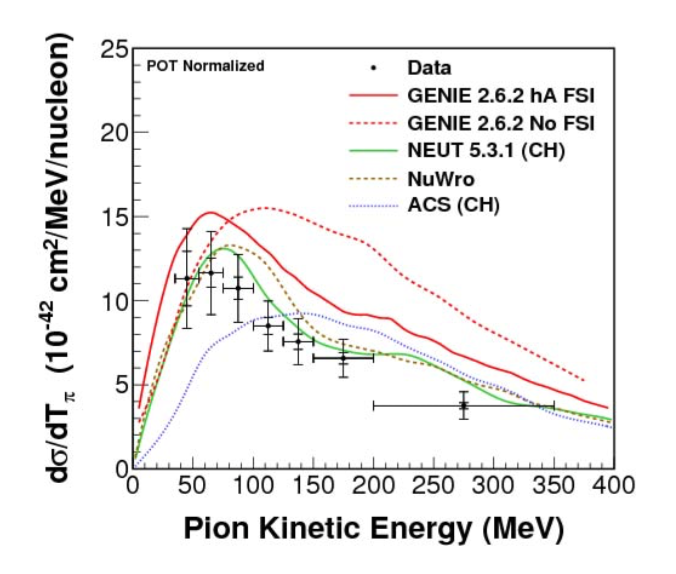
\includegraphics[width=0.98\textwidth]{./images/nuint/ccpi/minerva_cc1pi}\\
         {\scriptsize [Phys.Rev.D92, 092008 (2015)]}
      \end{center}
    \end{column}
    \begin{column}{0.50\textwidth}
      \begin{itemize}
        {\scriptsize
        \item Generator shape close to data
        \item As with MiniBooNE data, FSI stronly affects the prediction.
        \item Models with no FSI give wrong shape\\
        }
      \end{itemize}
      \begin{center}
         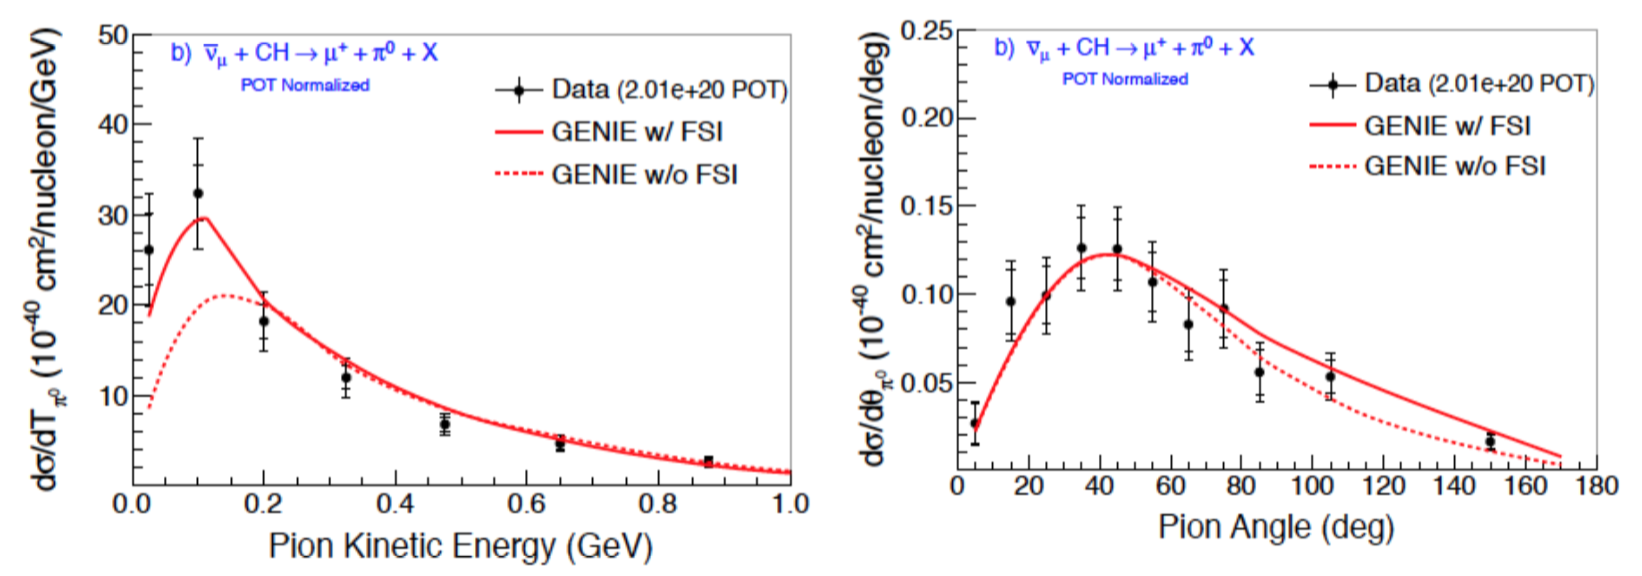
\includegraphics[width=0.98\textwidth]{./images/nuint/ccpi/minerva_CCpi0_2x}\\
      \end{center}
    \end{column}
  \end{columns}

\end{frame}


%
%
%
\begin{frame}{The single-$\pi$ puzzle}

  \begin{columns}
    \begin{column}{0.70\textwidth}
      \begin{center}
         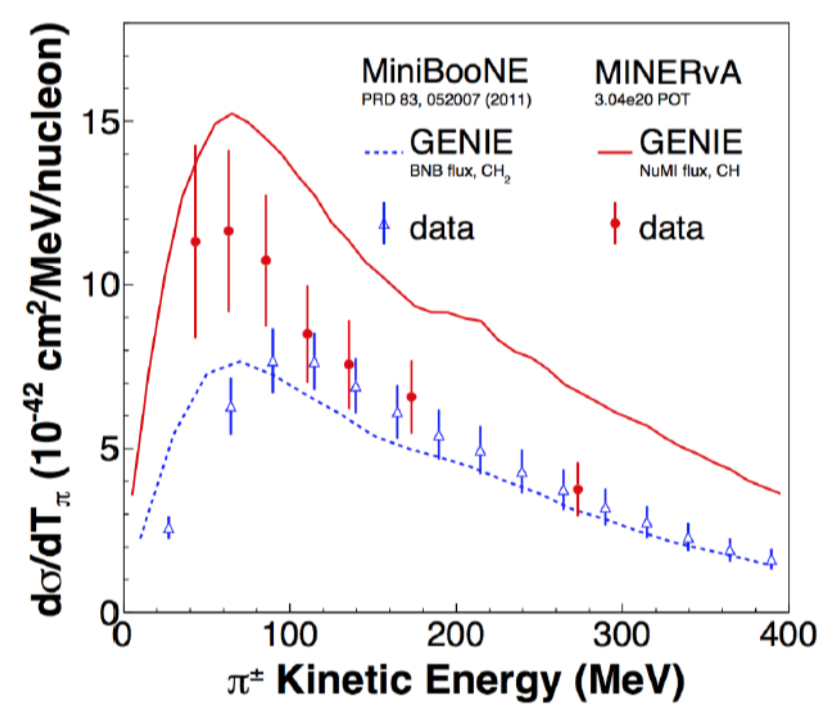
\includegraphics[width=0.98\textwidth]{./images/nuint/ccpi/cc1pi_mb_minerva_comp.png}\\
         {\scriptsize [Phys.Rev.D92, 092008 (2015)]}
      \end{center}
    \end{column}
    \begin{column}{0.30\textwidth}
      \begin{itemize}
      {\scriptsize
       \item Difficult to resolve the differences
       between MiniBooNE and MINERvA
       within our usual models.\\
       \vspace{0.4cm}
       \item This tension between MiniBooNE and MINERvA
       data is not understood.\\
      }
    \end{itemize}
    \end{column}
  \end{columns}

\end{frame}


%
% What you should know
%

\begin{frame}{What you should know}

\end{frame}


%
% What to read
%

\begin{frame}{What to read}

\begin{itemize}
{\scriptsize

\item
a

\vspace{0.1cm}
\item
b

}
\end{itemize}

\end{frame}
